\documentclass{beamer}

\input{slides-header.tex}

\title{Jedenáctá přednáška}
\subtitle{NAIL062 Výroková a predikátová logika}
\author{Jakub Bulín (KTIML MFF UK)}
% \institute{KTIML MFF UK}
\date{Zimní semestr 2024}


\begin{document}


\maketitle


\begin{frame}{Jedenáctá přednáška}

    \textbf{Program}
        \begin{itemize}            
            \item LI-rezoluce a Prolog
            \item elementární ekvivalence
            \item izomorfismus a konečné modely
            \item definovatelnost a automorfismy
            \item $\omega$-kategoricita a úplnost
        \end{itemize}

    \textbf{Materiály}

        \href{https://github.com/jbulin-mff-uk/nail062/raw/main/lecture/lecture-notes/lecture-notes.pdf}{\alert{\textbf{Zápisky z přednášky}}}, Sekce 8.7 z Kapitoly 8, Sekce 9.1-9.3 z Kapitoly 9
        %todo Prolog jako samostatná sekce?

\end{frame}


\section{8.7 LI-rezoluce (více podrobností ve skriptech, VL v Sekci 5.4)}


\begin{frame}{Lineární důkaz a LI-důkaz}

    \begin{itemize}[<+->]
        \item \alert{Lineární důkaz} klauzule $C$ z formule $S$ je konečná posloupnost
        $$
        \begin{bmatrix}
            C_0 \\
            B_0
        \end{bmatrix},
        \begin{bmatrix}
            C_1 \\
            B_1
        \end{bmatrix},\dots,
        \begin{bmatrix}
            C_n \\
            B_n
        \end{bmatrix},
        C_{n+1}
        $$
        kde: $B_0$ a $C_0$ jsou \myalertinline{varianty} klauzulí z $S$, $C_{n+1}=C$,
        \begin{itemize}
            \item $C_{i+1}$ je rezolventa $C_i$ a $B_i$
            \item $B_i$ \alert{varianta} klauzule z $S$ nebo $B_i=C_j$ pro nějaké $j<i$.
        \end{itemize}
        \item \alert{Lineární zamítnutí} $S$ je lineární důkaz $\square$ z $S$
        
        \item \alert{LI-důkaz} je lin. důkaz, kde vš. $B_i$ jsou varianty klauzulí z $S$
        \item $C$ \alert{LI-dokazatelná} z $S$, \alert{$S\proves_{LI}C$}, pokud existuje LI-důkaz
        \item $S$ je \alert{LI-zamítnutelná}, pokud $S\proves_{LI}\square$    
        \item korektnost (lineární i LI-rezoluce) je zřejmá
    \end{itemize}

    
\end{frame}


\begin{frame}{Úplnost LI-rezoluce pro Hornovy formule}

    \medskip

    \pause
    \myblock{
    \textbf{Věta (O úplnosti lineární rezoluce):}
        $C$ má lineární důkaz z $S$, právě když má rezoluční důkaz z $S$ (tj. $S\proves_R C$).
    }

    \pause
    \textbf{Důkaz:} \pause převodem na VL (Lifting lemma zachovává linearitu) \hfill\qedsymbol

    \bigskip

    \pause
    \myblock{
    \textbf{Věta (O úplnosti LI-rezoluce pro Hornovy formule):}
        Je-li Hornova formule $T$ splnitelná, a $T\cup\{G\}$ je nesplnitelná pro cíl $G$, potom $T\cup\{G\}\proves_{LI}\square$, a to LI-zamítnutím, které začíná cílem $G$.
    }
        
    \pause
    \textbf{Důkaz:} \pause úplnost ve VL + Herbrandova věta + Lifting lemma\hfill\qedsymbol

    \smallskip
    
    \pause
    \begin{itemize}[<+->]\small
        \item \alert{Hornova formule:} množina Hornových klauzulí
        \item \alert{Hornova klauzule:} nejvýše jeden pozitivní literál   
        \item \alert{Pravidlo:} klauzule s 1 pozitivním a alespoň 1 negativním literálem  
         
        \item \alert{Fakt:} pozitivní jednotková klauzule    
        \item \alert{Cíl:} neprázdná klauzule bez pozitivního literálu 
        \item \alert{Programové klauzule:} pravidla a fakta  
        \item \alert{Program}: Hornova formule obsahující jen programové klauzule
    \end{itemize}

\end{frame}


\begin{frame}[fragile]{Program v Prologu}

    \texttt{\small\setlength\tabcolsep{3pt}
    \begin{tabular}{lr}
        son(X,Y):-father(Y,X),man(X). 
        & 
       \alert{$\{son(X,Y),\neg father(Y,X),\neg man(X)\}$} 
        \\
        son(X,Y):-mother(Y,X),man(X).
        &
        \alert{$\{son(X,Y),\neg mother(Y,X),\neg man(X)\}$}
        \\
        man(charlie). 
        &
        \alert{$\{man(charlie)\}$}
        \\
        father(bob,charlie). 
        &
        \alert{$\{father(bob,charlie)\}$}
        \\
        mother(alice,charlie). 
        &
        \alert{$\{mother(alice,charlie)\}$}
        \\
        \\
        ?-son(charlie,X). 
        &
        \alert{$\{\neg son(charlie,X)\}$}
    \end{tabular}   
    }    

\end{frame}


\begin{frame}{LI-rezoluce v Prologu}

    \pause
    Platí v programu daný \alert{existenční dotaz},  \textcolor{blue}{$P\models(\exists X)son(charlie,X)$}?

    \medskip

    \pause
    \myblock{
        \textbf{Důsledek:}
        Pro program $P$ a cíl $G=\{\neg A_1,\dots,\neg A_k\}$ v proměnných $X_1,\dots,X_n$ jsou následující ekvivalentní:\pause
        \begin{itemize}
            \item $P\models(\exists X_1)\dots(\exists X_n)(A_1\wedge\dots\wedge A_k)$\pause
            \item $P\cup\{G\}$ má LI-zamítnutí začínající $G$
        \end{itemize}
    }

    \pause
    \vspace{-2pt}
    \textbf{Důkaz:} \pause Plyne z Důkazu sporem a Úplnosti LI-rezoluce pro Hornovy formule (Program je vždy splnitelný).\hfill\qedsymbol

    \bigskip

    \pause
    Je-li odpověď na dotaz kladná, chceme znát i \alert{výstupní substituci} $\sigma$, tj. složení unifikací z rez. kroků, zúžené na proměnné v $G$. Platí:
    $$
    P\models(A_1\wedge\dots\wedge A_k)\sigma
    $$

\end{frame}


\begin{frame}{Příklady}

    \pause
    \myexampleinline{\texttt{?-son(charlie,X).}}\pause

    \bigskip

    \hspace*{-1.13cm}\scalebox{0.82}{\begin{forest}
        for tree={math content,grow=west,l sep=5pt}
        [{\square}
            [,phantom]
            [{\{\neg father(X,c)\}}
                [,phantom]
                [{\{\neg father(X,c),\neg man(c)\}}
                    [,phantom]
                    [{\alert{\{\neg son(c,X)\}}}]
                    [{\{son(X',Y'),\neg father(Y',X'),\neg man(X')\}}, label=below:{\textcolor{blue}{$\{X'/c,Y'/X\}$}}]
                ]
                [{\{man(c)\}}, label=below:{\textcolor{blue}{$\emptyset$}}]                    
            ]
            [{\{father(b,c)\}}, label=below:{\textcolor{blue}{$\{X/b\}$}}]
        ]
    \end{forest}
    }

    \pause
    \myexampleinline{\texttt{X=bob}} \qquad výstupní substituce \textcolor{blue}{$\sigma=\{X/b\}$}\pause

    \bigskip

    \hspace*{-1.23cm}\scalebox{0.82}{
    \begin{forest}
        for tree={math content,grow=west,l sep=3pt}
        [{\square}
            [,phantom]
            [{\{\neg mother(X,c)\}}
                [,phantom]
                [{\{\neg mother(X,c),\neg man(c)\}}
                    [,phantom]
                    [{\alert{\{\neg son(c,X)\}}}]
                    [{\{son(X',Y'),\neg mother(Y',X'),\neg man(X')\}}, label=below:{\textcolor{blue}{$\{X'/c,Y'/X\}$}}]
                ]
                [{\{man(c)\}}, label=below:{\textcolor{blue}{$\emptyset$}}]                    
            ]
            [{\{mother(a,c)\}}, label=below:{\textcolor{blue}{$\{X/a\}$}}]
        ]
    \end{forest}
    }

    \pause
    \myexampleinline{\texttt{X=alice}} \qquad výstupní substituce \textcolor{blue}{$\sigma=\{X/a\}$}

\end{frame}


\section{ČÁST III -- POKROČILÉ PARTIE}


\section{\sc Kapitola 9: Teorie modelů}


\begin{frame}{Teorie modelů}

    \begin{itemize}[<+->]
        \item vztah mezi vlastnostmi teorií a tříd jejich modelů
        \item bližší matematice než informatice a aplikacím
        \item jen několik vybraných dostupných výsledků
        \item[+] co je třeba pro Gödelovy věty (Kapitola 10)
        \item[+] co se nevešlo jinam 
    \end{itemize}

\end{frame}


\section{9.1 Elementární ekvivalence}


\begin{frame}{Teorie struktury}

    \pause
    \myblock{
        \alert{Teorie struktury} $\A$ (v jazyce $L$):
        $$
        \Th(\A)=\{\varphi\mid\varphi\text{ je $L$-sentence a }\A\models\varphi\}
        $$
    }

    \medskip

    \pause
    Např.  pro \myexampleinline{standardní model aritmetiky} $\underline{\mathbb{N}}=\langle\mathbb{N},S,+,\cdot,0,\le\rangle$ říkáme $\Th(\underline{\mathbb{N}})$ \alert{aritmetika přirozených čísel}, je \alert{nerozhodnutelná} (neexistuje algoritmus, který pro každou $\varphi$ doběhne a odpoví, zda $T\models\varphi$)

    \medskip

    \pause
    \textbf{Pozorování:} Nechť $\A$ je $L$-struktura a $T$ je $L$-teorie.\pause
    \begin{itemize}
        \item $\Th(\A)$ je kompletní teorie\pause
        \item $\A\in\M_L(T)$ $\Rightarrow$ $\Th(\A)$ je (kompletní) jednoduchá extenze $T$\pause
        \item $\A\in\M_L(T)$, $T$ kompletní $\Rightarrow$ $\Th(\A)=\Conseq_L(T)\sim T$
    \end{itemize}

\end{frame}


\begin{frame}{Elementární ekvivalence}
    
    \pause
    \myblock{
        $L$-struktury $\A$ a $\B$ jsou \alert{elementárně ekvivalentní} (\alert{$\A\equiv \B$}), pokud v nich platí tytéž $L$-sentence, neboli: \myalertinline{ 
            $\A\equiv\B\ \Leftrightarrow\ \Th(\A)=\Th(\B)$ 
        }
    }

    \bigskip

    \pause
    Například pro \myexampleinline{
        $\langle\mathbb R,\leq\rangle$, 
        $\langle\mathbb Q,\leq\rangle$,
        $\langle\mathbb Z,\leq\rangle$
    }
    \pause
    \begin{itemize}[<+->]
        \item  \alert{$\langle\mathbb R,\leq\rangle\equiv\langle\mathbb Q,\leq\rangle$}: \pause snadno pomocí \alert{hustoty} \pause
        \item \alert{$\langle\mathbb Q,\leq\rangle\not\equiv\langle\mathbb Z,\leq\rangle$}: \pause v $\langle\mathbb Z,\leq\rangle$ má každý prvek bezprostředního následníka, v $\langle\mathbb Q,\leq\rangle$ ne, tedy $\varphi\in\Th(\langle\mathbb Z,\leq\rangle)\setminus\Th(\langle\mathbb Q,\leq\rangle)$ pro následující sentenci:\pause
        $$
        \varphi=(\forall x)(\exists y)(x\leq y\land \neg x=y\land(\forall z)(x\leq z\limplies z=x\lor y\leq z))
        $$        
    \end{itemize}

\end{frame}


\begin{frame}{Kompletní jednoduché extenze}

    \vspace{-6pt}

    \pause
    Pro teorii $T$ nás hlavně zajímá, jak vypadají modely.

    \pause
    \vspace{-6pt}
    \begin{itemize}
        \item $T$ je \alert{kompletní}, právě když má jediný model až na elementární ekvivalenci (všechny modely jsou elementárně ekvivalentní)\pause
        \item Modely $T$ až na elementární ekvivalenci jednoznačně odpovídají \alert{kompletním jednoduchým extenzím} $T$, ty jsou tvaru $\Th(\A)$ pro $\A\in\M(T)$, kde $\A\equiv\B\Leftrightarrow\Th(\A)=\Th(\B)$
    \end{itemize}
    
    \pause
    \myalert{Místo hledání modelů stačí najít kompletní jednoduché extenze!}

    \pause
    \myblock{
    \textbf{Motivace:} ukážeme, že lze-li \alert{efektivně popsat} všechny kompletní jednoduché extenze \alert{efektivně dané} teorie, potom je \alert{rozhodnutelná}.
    }   
    
    \pause
    \begin{itemize}
        \item algoritmus, který pro vstup $(i,j)$ vypíše $j$-tý axiom $i$-té kompletní jednoduché extenze (v nějakém očíslování)\pause
        \item algoritmus, který postupně vygeneruje všechny axiomy teorie
    \end{itemize}

    \pause
    Schopnost efektivně popsat kompletní jedn. extenze je vzácná, vyžaduje silné předpoklady, ale u mnoha důležitých teorií to lze. 

\end{frame}


\begin{frame}{Příklad: DeLO*}

    \pause
    \myexample{
        Teorie \alert{hustého lin. uspořádání (DeLO*)}  je extenze teorie uspořádání o \alert{linearitu} (\alert{dichotomii}), \alert{hustotu}, a někdy se přidává \alert{netrivialita}: 
        \begin{itemize}
            \item $x\leq y\lor y\leq x$
            \item ${x\leq y}\land{\neg\,x=y}\limplies(\exists z)(x\leq z\land z\leq y\land\neg\,z=x\land\neg\,z=y)$
            \item $(\exists x)(\exists y)(\neg\,x=y)$
        \end{itemize}        
    }

    \pause
    \myblock{
        \textbf{Tvrzení:} Buď $\varphi=(\exists x)(\forall y)(x\leq y)$ a $\psi=(\exists x)(\forall y)(y\leq x)$. Následující jsou právě všechny kompletní jednoduché extenze DeLO* (až na ekvivalenci):
        \begin{columns}\small
            \begin{column}{0.5\textwidth}
                \begin{itemize}
                    \item $\DeLO = \DeLO^*\ \cup \ \{\neg\varphi
                    ,\neg\psi\}$
                    \item $\DeLO^+ = \DeLO^*\ \cup \ \{\neg\varphi
                    ,\psi\}$                  
                \end{itemize}
            \end{column}
            \begin{column}{0.5\textwidth}
                \begin{itemize}                   
                    \item $\DeLO^- = \DeLO^*\ \cup \ \{\varphi
                    ,\neg\psi\}$
                    \item $\DeLO^\pm = \DeLO^*\ \cup \ \{\varphi
                    ,\psi\}$        
                \end{itemize}
            \end{column}
        \end{columns}
    }
    
    \pause
    Stačí ukázat, že jsou kompletní. Potom už je zřejmé, že žádná další kompletní jednoduchá extenze DeLO* nemůže existovat.\\  
    Jak ukážeme, kompletnost plyne z faktu, že jsou \alert{$\omega$-kategorické}, tj. mají jediný spočetný model až na \alert{izomorfismus}.
        
\end{frame}


\begin{frame}{Důsledky Löwenheim-Skolemovy věty bez rovnosti}

    \pause
    Připomeňme:

    \smallskip

    \pause
    \myblock{
        \textbf{Věta (L.-S. bez rovnosti):} 
        Ve spočetném jazyce bez rovnosti má každá bezesporná teorie spočetně nekonečný model.
    }

    \medskip

    \pause
    Jednoduchý důsledek:

    \smallskip

    \pause
    \myblock{
        \textbf{Důsledek:}
    Je-li $L$ spočetný bez rovnosti, potom ke každé $L$-struktuře existuje elementárně ekvivalentní spočetně nekonečná struktura.
    }

    \pause
    \textbf{Důkaz:} $\Th(\A)$ je bezesporná (má model $\A$), tedy dle L.-S. věty má spočetně nekonečný model $\B\models\Th(\A)$, to znamená $\B\equiv\A$.\hfill\qedsymbol

    \medskip

    \pause
    Bez rovnosti tedy nelze vyjádřit např. \myexampleinline{`model má právě 42 prvků'}.

\end{frame}


\begin{frame}{Důsledky Löwenheim-Skolemovy věty s rovností}

    \pause
    V důkazu L.-S. věty máme kanonický model pro bezespornou větev tabla z $T$ pro $\F\bot$; pro jazyk s rovností stačí faktorizovat dle $=^A$:

    \smallskip

    \pause
    \myblock{
        \textbf{Věta (L.-S. s rovností):}
        Ve spočetném jazyce s rovností má každá bezesporná teorie spočetný model (konečný, nebo nekonečný).
    }

    \medskip

    \pause
    I tato verze má snadný důsledek pro konkrétní struktury:

    \smallskip

    \pause
    \myblock{
        \textbf{Důsledek:}
        Je-li $L$ spočetný s rovností, ke každé \alert{nekonečné} $L$-struktuře existuje elem. ekvivalentní spočetně nekonečná struktura.
    }

    \smallskip

    \pause
    \textbf{Důkaz:}
    Mějme nekonečnou $L$-strukturu $\A$. Podobně jako v důkazu Důsledku bez rovnosti najdeme \alert{spočetnou} $\B\equiv\A$. 
    
    \pause
    Protože v $\A$ platí pro kažné $n\in\mathbb N$ sentence vyjadřující `existuje alespoň $n$ prvků' (což lze pomocí rovnosti snadno zapsat), platí i v $\B$, tedy $\B$ musí být nekonečná.\hfill\qedsymbol

\end{frame}


\begin{frame}{Spočetné algebraicky uzavřené těleso}

    \pause
    \begin{itemize}
        \item \alert{algebraicky uzavřené} těleso: každý polynom nenulového stupně v něm má kořen\pause
        \item $\mathbb Q$ není, $x^2-2$ nemá v $\mathbb Q$ kořen\pause
        \item $\mathbb R$ není, $x^2+1$ nemá v $\mathbb R$ kořen\pause
        \item $\mathbb C$ je algebraicky uzavřené, ale je nespočetné
    \end{itemize}

    \pause
    Algebraickou uzavřenost vyjádříme sentencemi $\psi_n$, pro $n>0$:
    
    \pause
    \myalertamsmath{
    $$
    (\forall x_{n-1})\dots(\forall x_0)(\exists y)(y^n+x_{n-1}\cdot y^{n-1}+\dots+x_1\cdot y + x_0) = 0
    $$
    }

    \pause
    kde $y^k$ je zkratka za term $y\cdot y \cdot\ \cdots\ \cdot y$

    \pause
    \myblock{
    \textbf{Důsledek:}
        Existuje spočetné algebraicky uzavřené těleso.
    }

    \smallskip

    \pause
    \textbf{Důkaz:}
    Dle Důsledku L.S. věty (s rovností) existuje spočetně nekonečná $\A\equiv\mathbb C$. Protože $\mathbb C$ je těleso a splňuje $\psi_n$ pro všechna $n>0$, je i $\A$ algebraicky uzavřené těleso.\hfill\qedsymbol

\end{frame}


\section{9.2 Izomorfismus struktur}


\begin{frame}{Definice izomorfismu}
    
    \pause
    \myblock{
        \alert{Izomorfismus} $\A$ a $\B$ (v $L=\langle\mathcal R,\mathcal F\rangle$) je bijekce $h\colon A\to B$ splňující:\pause
    \begin{itemize}
        \item pro každý ($n$-ární) $f\in\mathcal F$ a pro všechna $a_i\in A$:
        \vspace{-6pt}
        $$
        h(f^\A(a_1,\dots,a_n))=f^\B(h(a_1),\dots,h(a_n))
        $$
        \vspace{-24pt}\pause
        \item speciálně, je-li $c\in\mathcal F$ konstantní: $h(c^\A)=c^\B$\pause
        \item pro každý ($n$-ární) $R\in\mathcal R$ a pro všechna $a_i\in A$:
        \vspace{-6pt}
        $$
        R^\A(a_1,\dots,a_n)\ \text{ právě když }\ R^\B(h(a_1),\dots,h(a_n))
        $$
        \vspace{-24pt}
    \end{itemize}\pause
    Existuje-li, jsou \alert{izomorfní} (`\alert{via $h$}'), \alert{$\A\simeq\B$} (nebo \alert{$\A\simeq_h\B$}).\\
    \alert{Automorfismus} $\A$ je izomorfismus $\A$ a $\A$.\pause
    }
    \vspace{-6pt}
    \begin{itemize}
        \item tj. liší se jen `pojmenováním prvků'\pause
        \item relace `být izomorfní' je ekvivalence\pause
        \item např. potenční algebra \myexampleinline{\small
            $\underline{\mathcal P(X)}=\langle \mathcal P(X),-,\cap,\cup,\emptyset,X\rangle$
         }, $|X|=n$, \pause je izomorfní s {\small $\underline{2^n}=\langle \{0,1\}^n,-_n,\land_n,\lor_n,(0,\dots,0),(1,\dots,1)\rangle$} (operace po složkách) via \alert{$h(A)=\chi_A$} (charakt. vektor $A\subseteq X$)
    \end{itemize}

\end{frame}


\begin{frame}{Izomorfismus zachovává sémantiku \& vztah $\simeq$ a $\equiv$}
    
    \pause
    \myblock{
        \textbf{Tvrzení:} Bijekce $h\colon A\to B$ je izomorfismus $\A$ a $\B$, právě když:\pause
        \begin{enumerate}[(i)]
            \item pro každý term $t$ a $e:\Var\to A$:\hfill
            \alert{$h(t^\A[e])=t^\B[e\circ h]$}\pause
            \item pro každou $\varphi$ a $e:\Var\to A$:\hfill
            \alert{$\A\models\varphi[e]\Leftrightarrow\B\models\varphi[e\circ h]$}
        \end{enumerate}
    }

    \pause
    \textbf{Důkaz:} \pause \alert{\Large$\Rightarrow$} snadno indukcí podle struktury termu resp. formule

    \pause
    \alert{\Large$\Leftarrow$} je-li $h$ bijekce splňující (i)\&(ii), dosazení $t=f(x_1,\dots,x_n)$ resp. $\varphi=R(x_1,\dots,x_n)$ dává vlastnosti z definice izomorfismu \hfill\qedsymbol

    \pause
    \myblock{
        \textbf{Důsledek:} 
        $\A\simeq\B\ \Rightarrow\ \A\equiv\B$.
    }
    \pause
    \textbf{Důkaz:} pro každou sentenci $\varphi$ máme z (ii) $\A\models\varphi\Leftrightarrow\B\models\varphi$\hfill\qedsymbol
    
    \pause
    Naopak obecně ne, \myexampleinline{
        $\langle\mathbb Q,\leq \rangle\equiv\langle\mathbb R,\leq\rangle$, $\langle\mathbb Q,\leq \rangle\not\simeq \langle \mathbb R,\leq\rangle$
    } \pause Platí ale:

    \pause
    \myblock{\textbf{Tvrzení:}
        Jsou-li $\A,\B$ konečné v jazyce s rovností, potom
        \vspace{-9pt}
        $$
        \A\simeq\B\ \Leftrightarrow\ \A\equiv\B
        $$
        \vspace{-20pt}        
    }

    \pause
    \myblock{
        \textbf{Důsledek}
        Pokud má kompletní teorie v jazyce s rovností konečný model, potom jsou všechny její modely izomorfní.
    }   
    
\end{frame}


\begin{frame}{Důkaz $\equiv\ \Rightarrow\ \simeq$ pro konečné struktury s rovností}
    
    \pause
    \vspace{-6pt}
    Díky $=$ vyjádříme ``existuje právě $n$ prvků'', z toho plyne \alert{$|A|=|B|$}. \pause 
    Buď $\A'$ expanze $\A$ o jména prvků, v jazyce $L'=L\cup\{c_a\mid a\in A\}$. Ukážeme: $\B$ \alert{lze expandovat} na $L'$-strukturu $\B'$ \alert{že $\A'\equiv \B'$}.\pause Potom je \alert{$h(a)= c_a^{\B'}$} izomorfismus $\A'$ a $\B'$, i pro $L$-redukty $\A\simeq\B$. \pause
    
    Stačí ukázat, že \alert{pro $c_a^{\A'}=a\in A$ existuje $b\in B$} tak, že expanze o interpretaci konstantního symbolu $c_a$ splňují \alert{$\langle \A,a\rangle\equiv\langle\B,b\rangle$}. \pause 
    
    Buď $\Omega$ množina `\alert{vlastností prvku $a$}', \pause tj. formulí $\varphi(x)$ splňujících $\langle \A,a\rangle \models \varphi(x/c_a)$, neboli $\A\models \varphi[e(x/a)]$. \pause Protože je $A$ konečná, existuje \alert{konečně mnoho $\varphi_1(x),\dots,\varphi_m(x)$} tak, že pro každou $\varphi \in \Omega$ existuje $i$ takové, že $\A\models \varphi\liff\varphi_i$. \pause Potom i $\B\models\varphi\liff\varphi_i$. %(neboť $\A\equiv\B$, stačí vzít generální uzávěr, což je sentence).
    
    \pause
    Protože v $\A$ platí sentence \alert{$(\exists x)\bigwedge_{i=1}^m\varphi_i$} (je splněna díky $a\in A$) a $\B\equiv\A$, máme i $\B\models (\exists x)\bigwedge_{i=1}^m\varphi_i$. \pause Neboli existuje $b\in B$ takové, že $\B\models \bigwedge_{i=1}^m\varphi_i[e(x/b)]$. \pause Tedy pro každou $\varphi\in \Omega$ platí $\B\models \varphi[e(x/b)]$, tj. $\langle\mathcal{B},b\rangle\models \varphi(x/c_a)$, z toho $\langle \A,a\rangle\equiv\langle\B,b\rangle$.\hfill\qedsymbol

\end{frame}


\begin{frame}{Definovatelnost a automorfismy}

    \pause
    definovatelné množiny jsou \alert{invariantní} na automorfismy (např. automorfismus grafu musí zobrazit trojúhelník na trojúhelník):

    \medskip

    \pause
    \myblock{
        \textbf{Tvrzení:}\pause
        Je-li $D\subseteq A^n$ definovatelná v $\A$, potom pro každý automorfismus $h\in\Aut(\A)$ platí $h[D]=D$ (kde $h[D]$ značí $\{(h(\overline{a})\mid\overline{a}\in D\}$).
    
        \pause
        Je-li definovatelná s parametry $\overline{b}$, platí to pro automorfismy identické na $\overline{b}$ (tj. $h(\overline{b})=\overline{b}$ neboli $h(b_i)=b_i$ pro všechna $i$).
    }

    \pause
    \textbf{Důkaz:}
    Ukážeme jen verzi s parametry. Nechť $D=\varphi^{\A,\overline{b}}(\overline{x},\overline{y})$. Potom pro každé $\overline{a}\in A^n$ platí následující ekvivalence:\pause
    \begin{align*}
    \overline{a}\in D\ 
    &\Leftrightarrow\ \A\models \varphi[e(\overline{x}/\overline{a},\overline{y}/\overline{b})]\\
    &\Leftrightarrow\  \A\models \varphi[(e\circ h)(\overline{x}/\overline{a},\overline{y}/\overline{b})]\\
    &\Leftrightarrow\ \A\models \varphi[e(\overline{x}/h(\overline{a}),\overline{y}/h(\overline{b}))]\\
    &\Leftrightarrow\ \A\models \varphi[e(\overline{x}/h(\overline{a}),\overline{y}/\overline{b})]\\
    &\Leftrightarrow\ h(\overline{a})\in D.
    \end{align*}

    \vspace{-0.85cm}
    \hfill\qedsymbol    

\end{frame}


\begin{frame}{Příklad}

    \vspace{6pt}

    \begin{columns}

        \begin{column}{0.8\textwidth}            
            Množiny definovatelné s parametrem $0$, $\mathrm{Df}^1(\mathcal G,\{0\})$? Jediný netriviální automorfismus zachovávající $0$: \alert{$h(i)=(5-i) \bmod 5$}, orbity $\{0\}$, $\{1,4\}$, a $\{2,3\}$. Tyto množiny jsou definovatelné:            
        \end{column} 

        \begin{column}{0.2\textwidth}            
            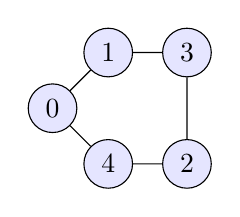
\begin{tikzpicture}[every node/.style={circle,fill=blue!10,draw,minimum size=0.4cm,node distance=1cm}]
                \node (1) {$1$};
                \node[below left of=1](0) {$0$};
                \node[below right of=0] (4) {$4$};
                \node[right of=4] (3) {$2$};
                \node[right of=1] (2) {$3$};
                \path[draw] (0) -- (1) -- (2) -- (3) -- (4) -- (0);
            \end{tikzpicture}                        
        \end{column}

    \end{columns}

    \pause
    \begin{itemize}
        \item $\{0\}$ formulí $x=y$, tj. $(x=y)^{\mathcal G,\{0\}}=\{0\}$\pause
        \item $\{1,4\}$ lze definovat pomocí $E(x,y)$\pause
        \item $\{2,3\}$ formulí $\neg E(x,y)\land \neg x=y$\pause
    \end{itemize}
    $\mathrm{Df}^1(\mathcal G,\{0\})$ je podalgebra $\underline{\mathcal P(V(\mathcal G))}$, tedy uzavřená na doplněk, sjednocení, průnik, obsahuje $\emptyset$ a $V(\mathcal G)$. Podalgebra generovaná $\{\{0\},\{1,4\},\{2,3\}\}$ už ale obsahuje všechny podmnožiny zachovávající automorfismus $h$. Dostáváme:\pause
    \begin{align*}        
        \mathrm{Df}^1(\mathcal G,\{0\})=\{&\emptyset, \{0\}, \{1,4\}, \{2,3\}, \{0,1,4\}, \{0,2,3\}, \\ &\{1,4,2,3\}, \{0,1,2,3,4\}\}        
    \end{align*}
    
\end{frame}


\section{9.3 $\omega$-kategorické teorie}


\begin{frame}{$\omega$-kategorické teorie}

    \pause
    \vspace{-8pt}
    \alert{Izomorfní spektrum} $T$ je počet modelů $T$ kardinality $\kappa$ až na $\simeq$.\\
    $T$ je \alert{$\kappa$-kategorická} pokud $I(\kappa,T)=1$, \alert{$\omega$-kategorická} má-li jediný spočetně nekonečný model až na izomorfismus.

    \pause
    \vspace{-3pt}
    \myblock{
        \textbf{Tvrzení:}
        Teorie DeLO je $\omega$-kategorická.
    }
    \pause
    \textbf{Důkaz:}
    Buďte $\A,\B$ spočetně nekonečné modely, $A=\{a_i\mid i\in\mathbb N\}$, $B=\{b_i\mid i\in\mathbb N\}$. Z hustoty najdeme indukcí $h_0\subseteq h_1\subseteq h_2\subseteq\dots$ prosté parciální fce z $A$ do $B$ zach. usp., $\{a_0,\dots,a_{n-1}\}\subseteq\dom h_n$, $\{b_0,\dots,b_{n-1}\}\subseteq\rng h_n$. Potom $\A\simeq\B$ via $h=\bigcup_{n\in\mathbb N}h_n$.
    \hfill\qedsymbol

    \pause
    \myblock{
        \textbf{Důsledek:}
        Izomorfní spektrum teorie DeLO*:
        \vspace{-3pt}
        \begin{itemize}
            \item $I(\kappa,DeLO^*)=0$ pro $\kappa\in\mathbb{N}$
            \item $I(\omega,DeLO^*)=4$
        \end{itemize}      
        \vspace{-3pt}
        \pause
        Spočetné modely až na izomorfismus jsou například:
        \vspace{-9pt}
        $$ 
        \mathbb Q=\langle \mathbb Q,\leq\rangle\simeq\mathbb Q\upharpoonright(0,1), \ \mathbb Q\upharpoonright(0,1], \ \mathbb Q \upharpoonright [0,1), \ \mathbb Q \upharpoonright [0,1]
        $$
        \vspace{-20pt}
    }
    \pause
    \textbf{Důkaz:}
    Husté uspořádání nemůže být konečné. Izomorfismus zobrazí minimum na minimum a maximum na maximum.
    \hfill\qedsymbol

\end{frame}


\begin{frame}{$\omega$-kategorické kritérium kompletnosti}

    %\alert{$\omega$-kategoricita} je zeslabení pojmu \alert{kompletnosti}

    \pause
    \myblock{
        \textbf{Věta:}
        Buď $T$ $\omega$-kategorická ve spočetném jazyce $L$. Je-li\pause
        \begin{enumerate}[(i)]
            \item $L$ bez rovnosti, nebo\pause
            \item $L$ s rovností a $T$ nemá konečné modely,\pause
        \end{enumerate}
        potom je $T$ kompletní.
    }

    \pause
    \textbf{Důkaz:}\pause
    \alert{(i)} Důsledek L.-S. věty bez rovnosti říká, že každý model je elementárně ekvivalentní nějakému spočetně nekonečnému, ten je ale až na izomorfismus jediný.\pause
    
    \alert{(ii)} \pause Důsledek L.-S. věty s rovností podobně říká, že všechny nekonečné modely jsou elementárně ekvivalentní. Mohla by mít elementárně neekvivalentní konečné modely, to jsme ale zakázali. \hfill\qedsymbol

    \medskip

    \pause
    \myblock{
        \textbf{Důsledek:}
        $\DeLO$, $\DeLO^+$, $\DeLO^-$, a $\DeLO^\pm$ jsou kompletní, jsou to všechny (navzájem neekvivalentní) kompletní jedn. extenze $DeLO^*$.
    }

    \pause
    Analogické kritérium platí i pro kardinality $\kappa$ větší než $\omega$.

\end{frame}


\end{document}


